\chapter{Probleme in der Umsetzung}
In diesen Kapitel möchte ich auf Probleme mit der Entwicklung eines Videospiels mit Hilfe von KI-Systemen eingehen.

\section{Ablenkung und Abschweifung}
In \ref{chatgpt-ptompt-Midjourney-04} Umsetzung habe ich mir einen Prompt für Midjourne ausgeben lassen für einen Abentuerer mit Fuchskopf. Der Gund warum ich ChatGPT nicht aufgefordert habe mir eine Ausgabe von Martin Luther ausgeben zu lasse, das ich abgelenkt war und mir spontan die Idee von einem Abenteurer mit Fuchskopf gekommen ist.
Diese vermeidbare Grenzenlosigkeit, verleitet uneffektiv mit dem Werkzeug zu arbeiten und es kann passieren das KI-Werkzeuge persönlich mehr als Spielzeuge wahrgenommen werden, anstatt Werkzeuge die ein Workflow bereichern kann um Zeit und Geld zu sparen.

\section{Einarbeitungszeit}
KI-Systeme benötigen Einarbeitungszeit. Bis ich PIFuHD zum laufen gebracht habe, vergingen Tage mit neuen versuchen. Abildung \ref{erstemalpifuhdblender} zeigt das erste Ergebnis was ich mit der Kombination Midjourney und PIFuHD erzeugt habe.
\begin{figure}
	\centering
	\begin{minipage}[t]{0.45\linewidth}
		\centering
		\includegraphics[width=6.405cm\linewidth]{BilderFuerBA/ersteMalPIFuHD}
		\caption{Midjourney: Erstes Testbild für PIFuHD}
		\label{erstemalpifuhd}
	\end{minipage}
	\hfill
	\begin{minipage}[t]{0.45\linewidth}
		\centering
		\includegraphics[width=6.405cm\linewidth]{BilderFuerBA/ErsteMalPIFuHDblender}
		\caption{Blender: Erstes 3D-Modell von PIFuHD}
		\label{erstemalpifuhdblender}
	\end{minipage}
\end{figure}
Dieser Test hat mir gezeigt, das es möglich ist, durch MIdjourney generierte Bilder für
\section{weis nicht alles}
Chat GPT besitzt eine sehr natürliche Form der Benutzung - die natürlicher Sprache. Midjourney hingegen verlangt eine Kommunikation in Stich- beziehungsweise Schlagworten.
\\
Einer meiner Ersten Gedanken war es, ChatGPT so zu verwenden, das ChatGPT mein Dolmetscher ist. In meiner Vorstellung erkläre ich ChatGPT in Natürlicher Sprache was ich für Bilder von Midjourney haben möchte, und ChatGPT  gibt mir den Passenden Prompt für Midjourney.
\\
Dieser Gedanke hat leider nicht so gut funktioniert wich es mir gedacht habe. Das lag im ersten Moment daran, das ChatGPT nicht richtig darauf trainiert ist, Midjourney-Prompts zu erzeugen. Weitere Probleme entstand, das ich zwei werkzeuge gleichzeitige bedienen musste, obwohl ich nur ein KI-System benötigte um Bilder zu generieren.
\\
Ich bin dann zu dem Schluss gekommen, nicht mehr mit ChatGPT zu arbeiten, und habe selständig meine Prompts für Midjourney geschrieben und verändert.
\\
Mein Erste Gedanke und Ansatz in der Richtung war es, das ChatGPT eine Art Dolmecer zwischen mir als Anwender und Midjourney steht.
Midjourney-Prompts sind weniger in Natürlicher Sprache verfasst, sonder eher mehr in Stichworten strukturiert.
Meine erster Gedanke hat sich an dieser Stelle als falsch erwiesen. Die Lösung dieses Problems war es durch einen einfachen Prompt, ChatGPT eine Midjourneyformel beizubringen, was gut funktioniert hat.
Das Problem was anschließend daraus entstand, ist Das ChatGPT immernoch nicht gute Midjourney-Promts erzeugt.
Als ich für dieses Problem keine Lösung entwickeln konnte, und auch keinen weiteren Lösungsansatz gefunden habe. blieb mir nur noch die Möglichkeit meine Midjourney-Prompts selber zu schreiben und an den gewünschten stellen etwas zu verändern was mich näher zu meinem Ziel bringt.
Abbildung \ref{ChatGPT_erster_Versuch_Midjourney_Promt} zeigt das ich gerne
\section{konsistenz}
Ein Problem möchte ich mit dem Begriff Konsistenz beschreiben.
KI-Systeme verändern sich mit der Zeit, das bedeutet, das ein Prompt heute nicht das gleiche Ergebnis bring wie in einem Jahr.
Das bedeutet, das neben der Einarbeitung in KI-Systeme auch eine
\begin{figure}
	\centering
	\begin{minipage}[t]{0.45\linewidth}
	\centering
	\includegraphics[width=6.405cm\linewidth]{BilderFuerBA/Sonstiges/mlAltSelberSeed}	
	\end{minipage}
	\hfill
	\begin{minipage}[t]{0.45\linewidth}
	\centering
	\includegraphics[width=6.405cm\linewidth]{BilderFuerBA/Sonstiges/mlNeuSelberSeed}
	\end{minipage}
	\caption{Midjourney: Vergleich Juni 2023 und Oktober 2023 mit Midjourney}
	\label{MLaltSelberSeedUndVersion}
\end{figure}
\\
In Abbildung \ref{MLaltSelberSeedUndVersion} sehen wir unterschiedliche Ausgaben von Midjourney. Die Prompts sind die Selben mit dem gleichen Version und dem gleichen Seed.
\\
Aus diesem Experiment zeigt, das eine Reproduzierbarkeit von Ergebnisen sehr schwer bis unmöglich ist.

\section{Urheberrecht}
%https://docs.midjourney.com/docs/terms-of-service
Darf ich das Ausgabematerial benutzen oder nicht? 
\\
Der Erste Blick um diese Frage zu beantworten ist ein Blick in die jeweiligen Geschäftsbedingungen. Desweiteren ist man gut beraten mit einem Anwalt darüber zu reden.
\\
Zum Beispiel bezahle ich eien monatliche gebühr von 10 US \$. MIt dieser Subscription erhalte ich General commercial terms. Diese Term erlauben mir laut Midjourney mit den Bilder zu machen was ich möchte, aber ich besitze diese Werke nicht.
\\
%https://www.rollingstone.de/george-r-r-martin-und-john-grisham-klagen-gegen-openai-2639243/
%https://www.golem.de/news/stable-diffusion-und-midjourney-urheberrechtsklage-gegen-ki-bildgeneratoren-2301-171242.html
Während meiner Arbeit an dem Prototypen sind mir drei Nachrichtenmeldungen besonders aufgefallen, rund um das Thema Uhrheberrecht.
\\
Laut golem.de haben Künstler Klage gegen KI-Bildgeneratoren wie Midjourney eingereicht. Hintergrund ist, das die Künstler ihre Rechte im Urheberschutz verletzt sehen.
\begin{figure}
	\centering
	\begin{minipage}[t]{0\linewidth}
		\centering
		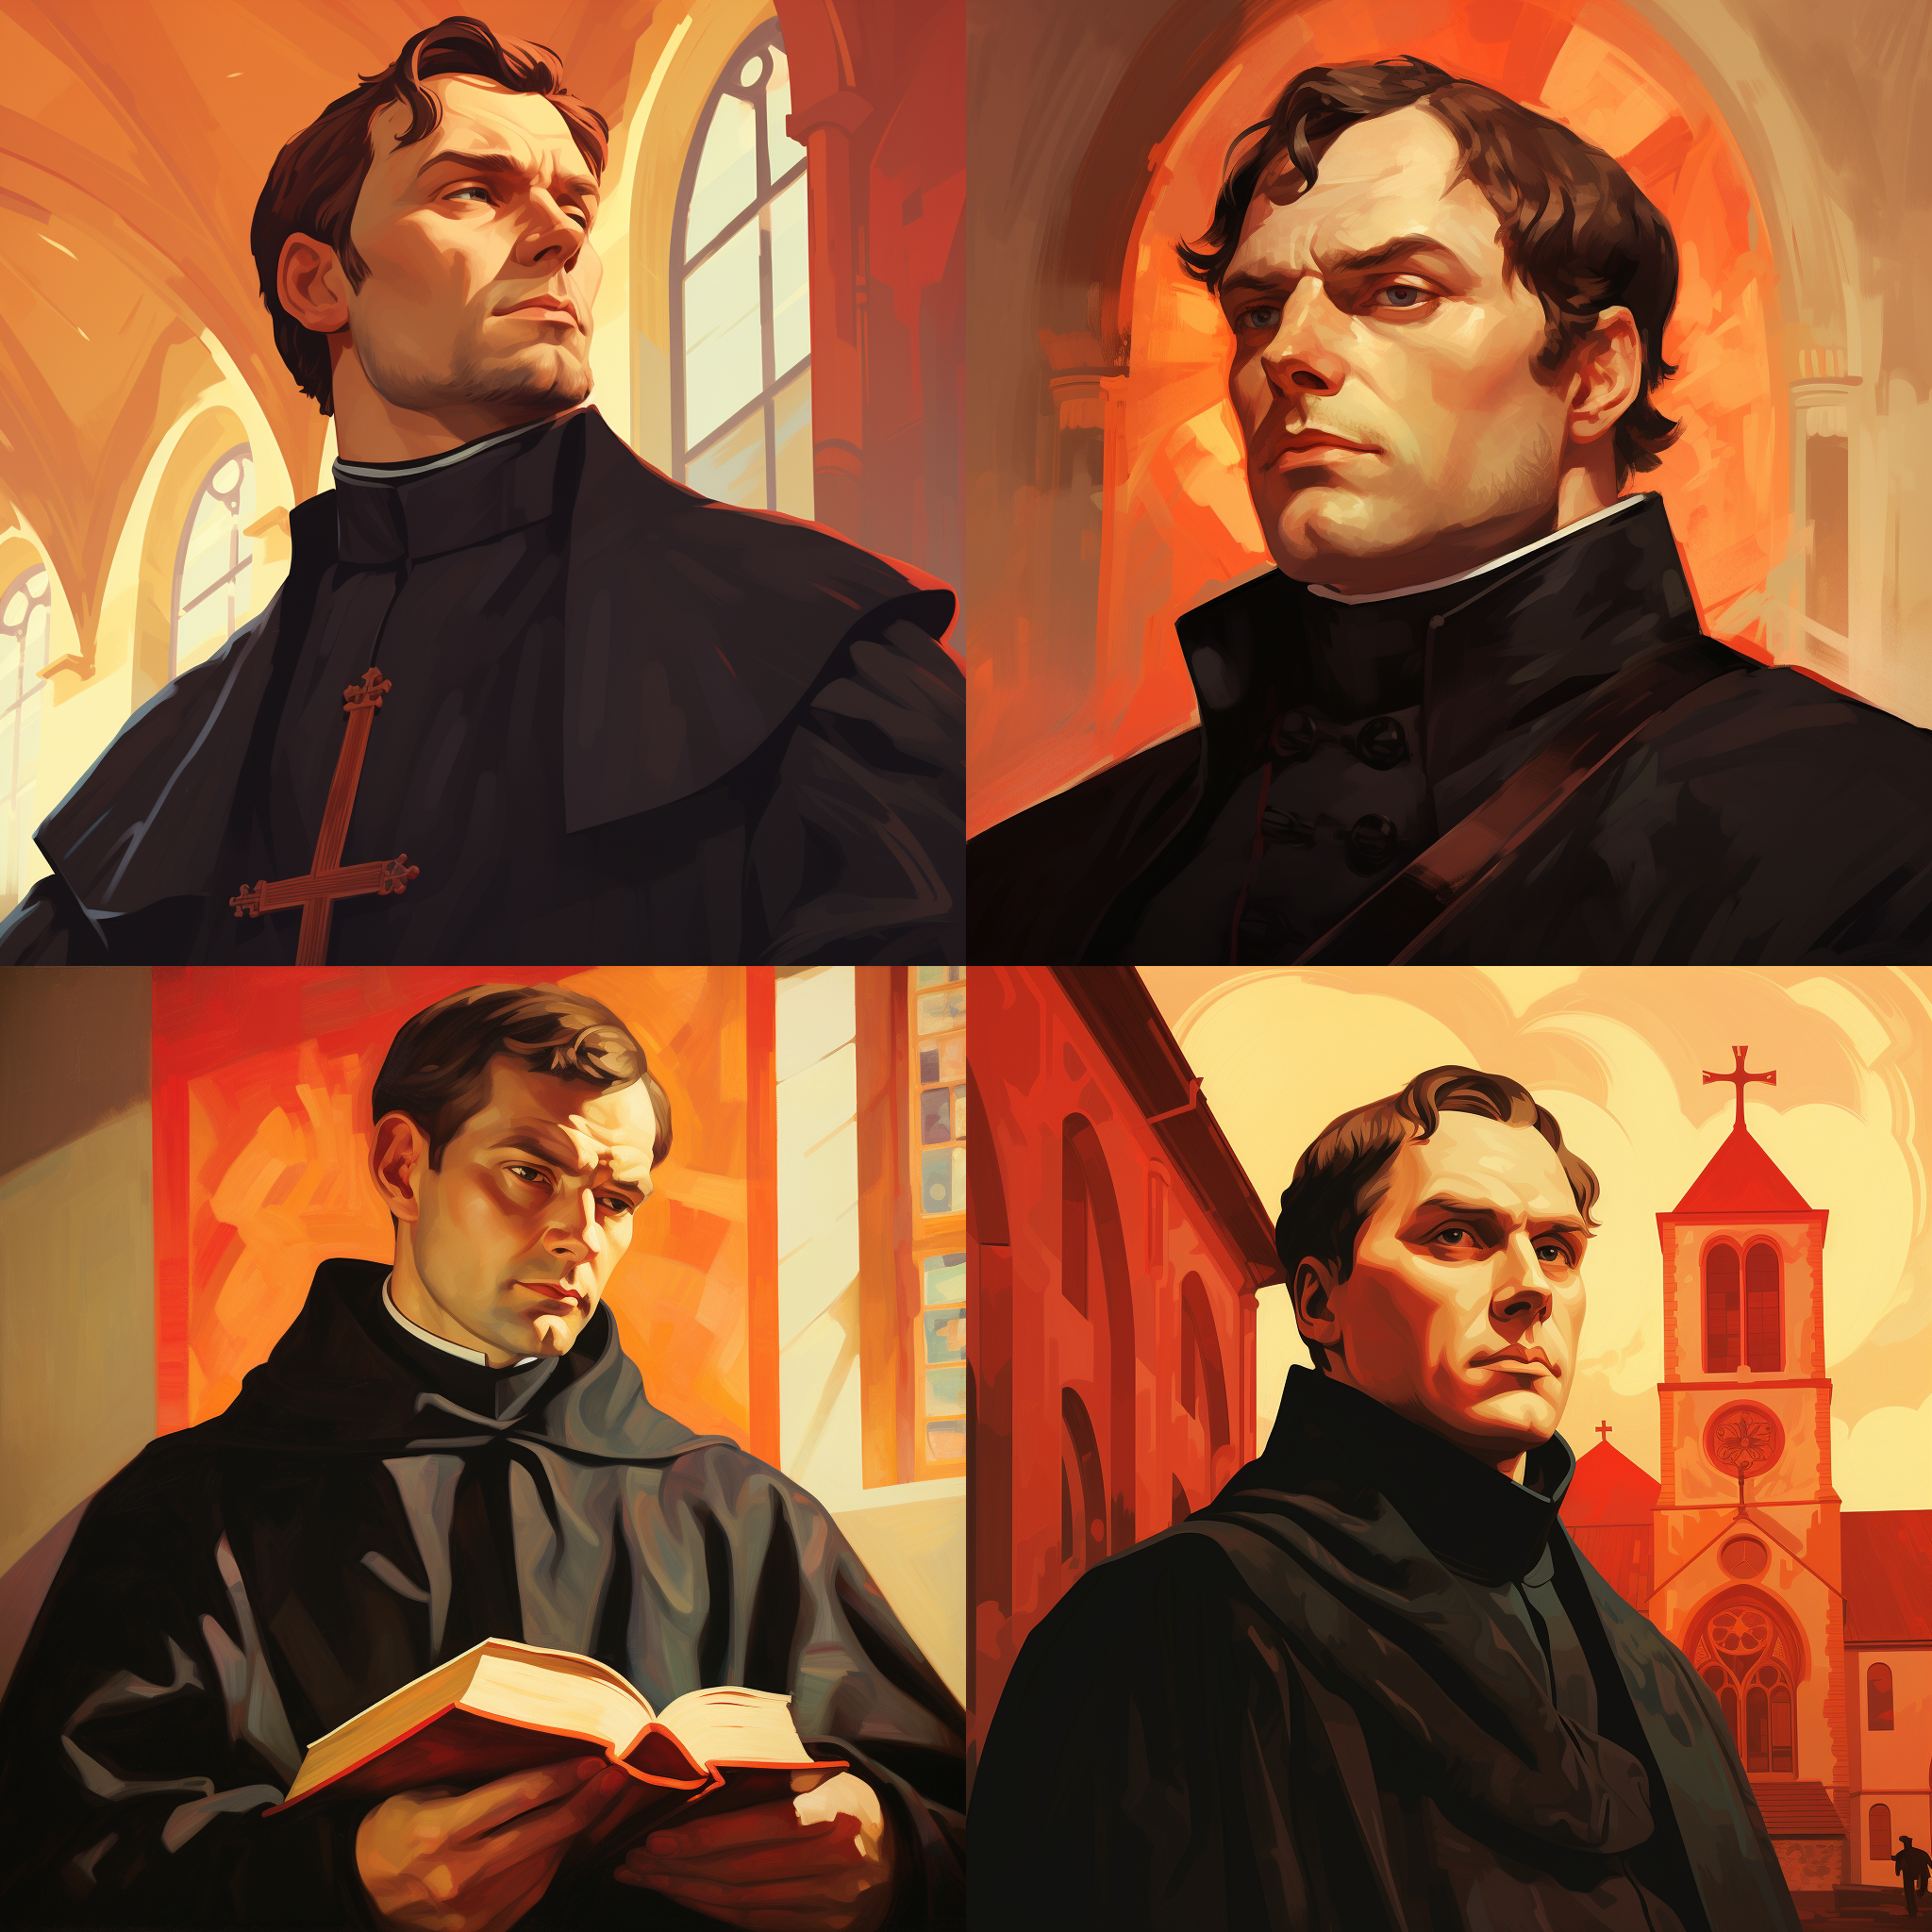
\includegraphics[width=4cm]{BilderFuerBA/Sonstiges/Martin_Luther_in_style_of_Ilya_Kuvshinov}
	\end{minipage}
	\hfill
	\begin{minipage}[t]{0.3855\linewidth}
		\centering
		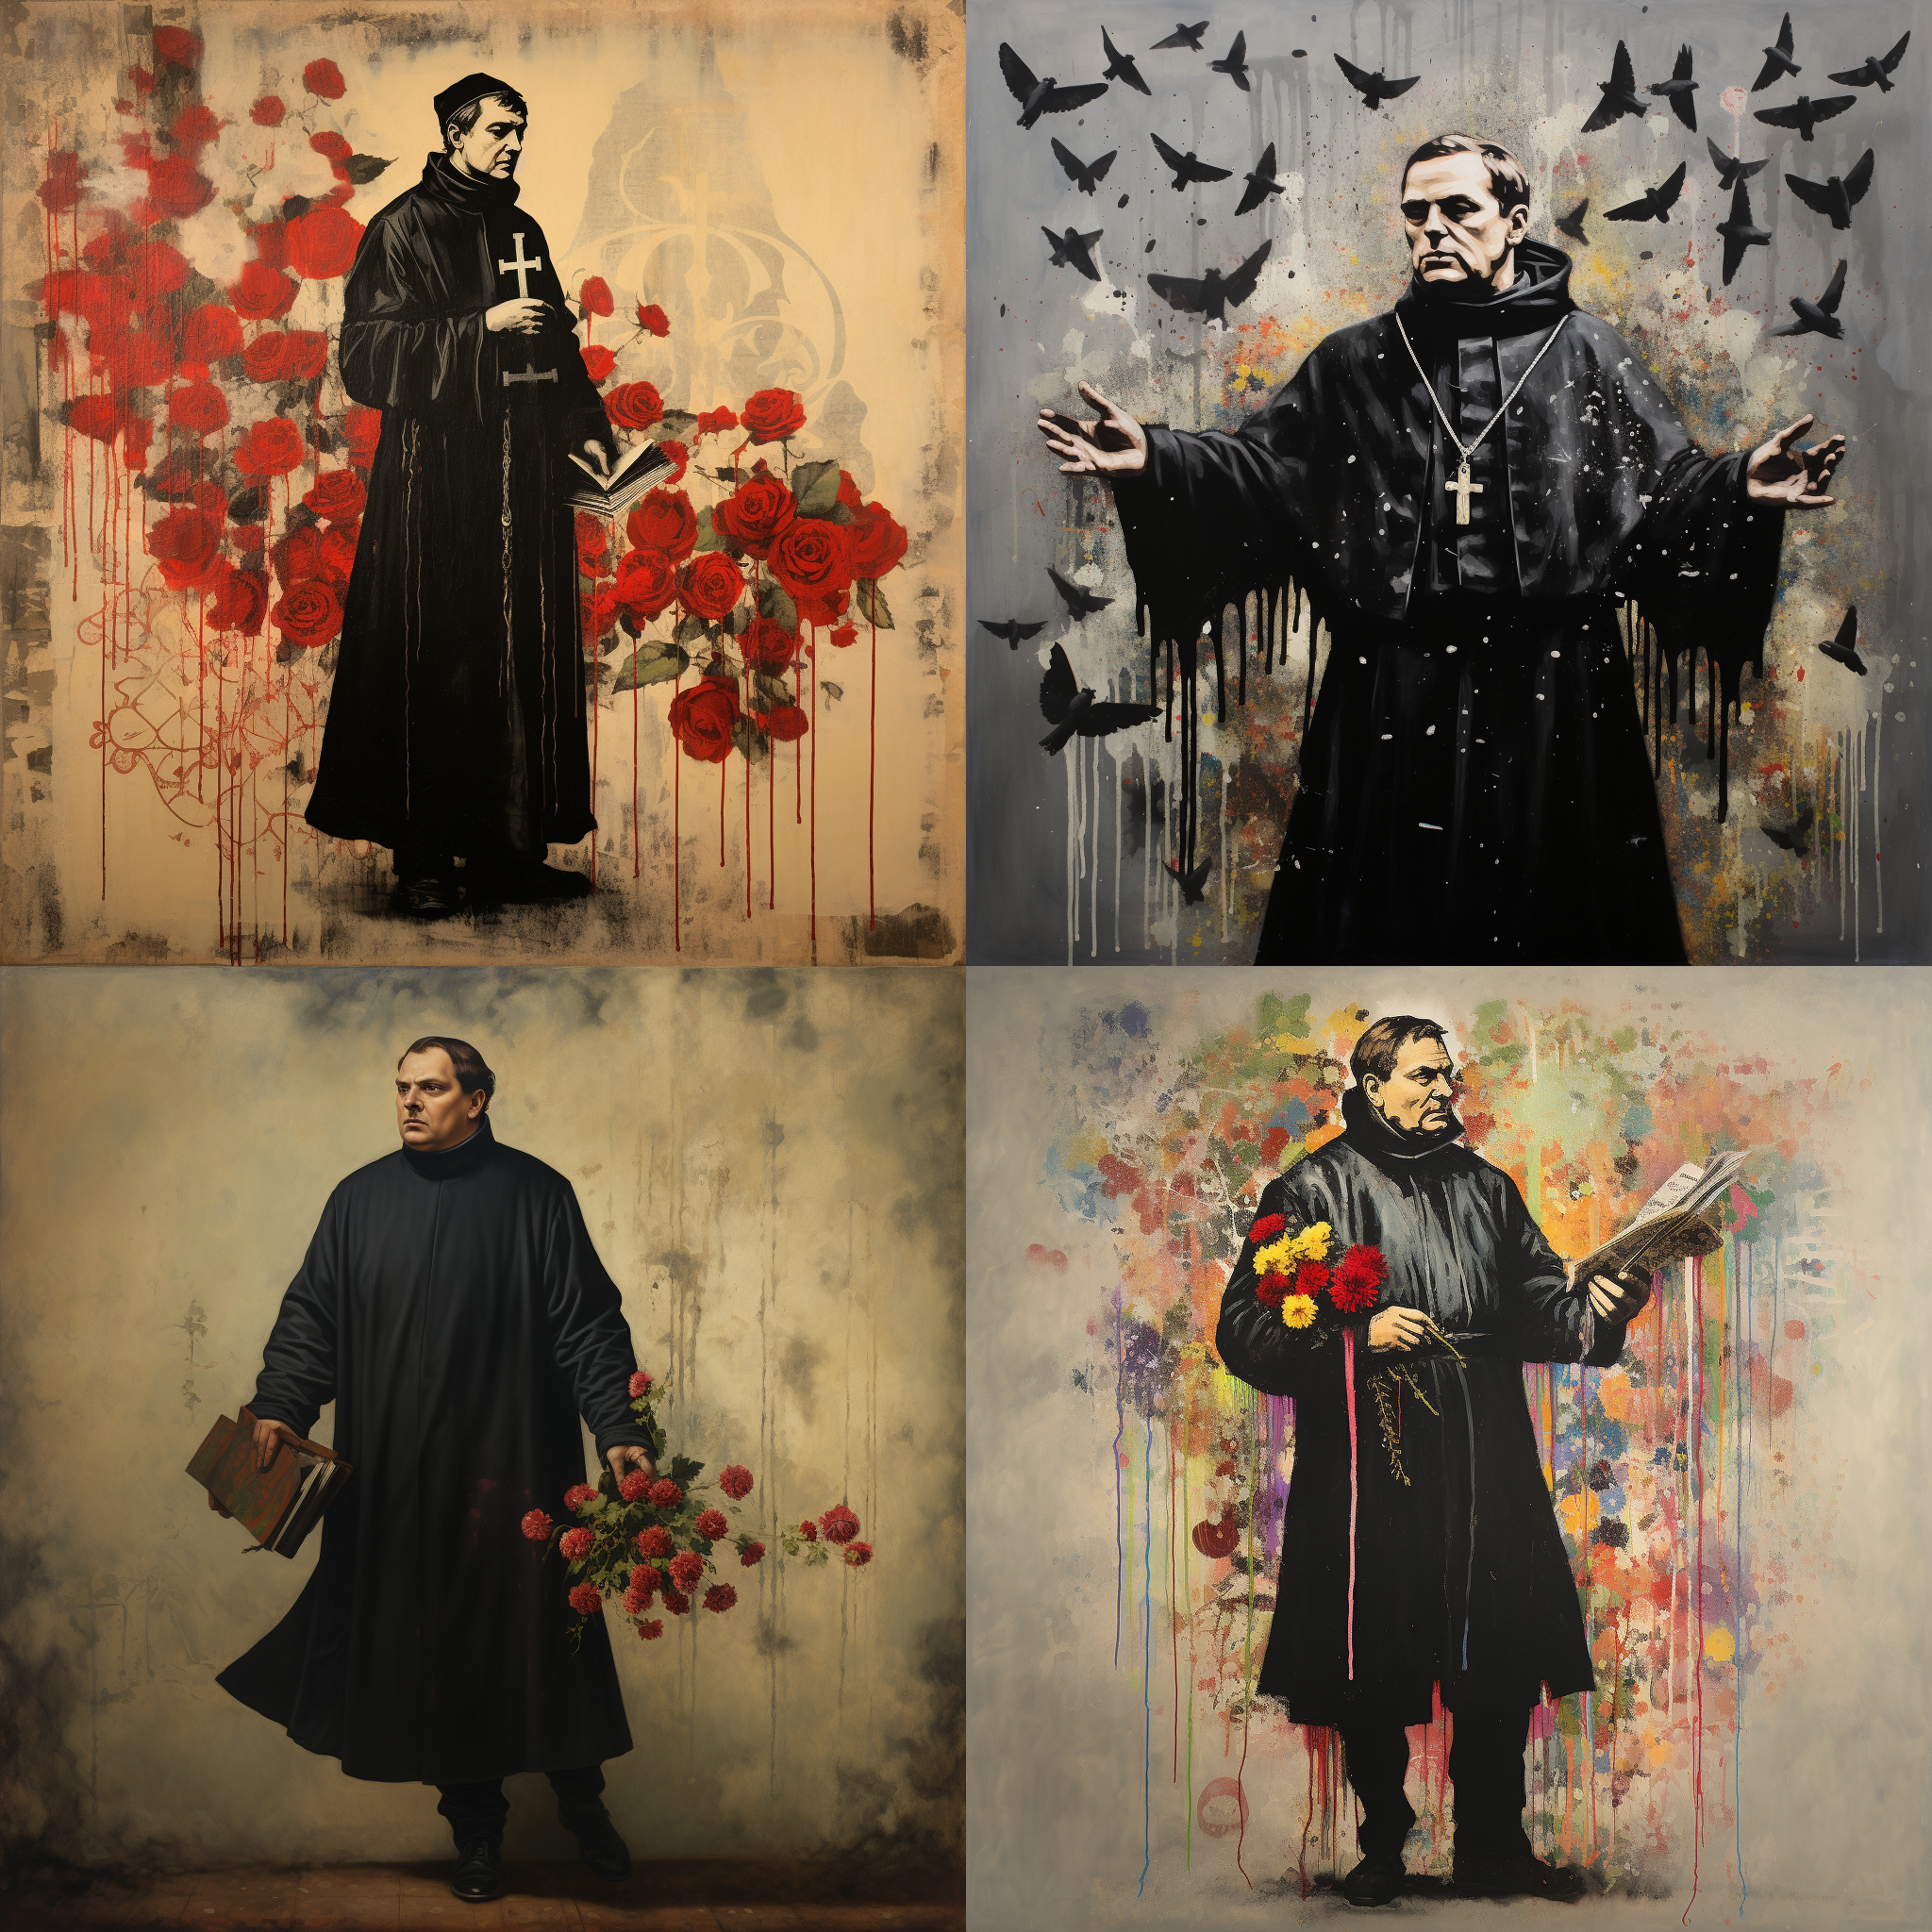
\includegraphics[width=4cm]{BilderFuerBA/Sonstiges/Martin_Luther_in_style_of_banksy}
	\end{minipage}
	\begin{minipage}[t]{0.3\linewidth}
		\centering
		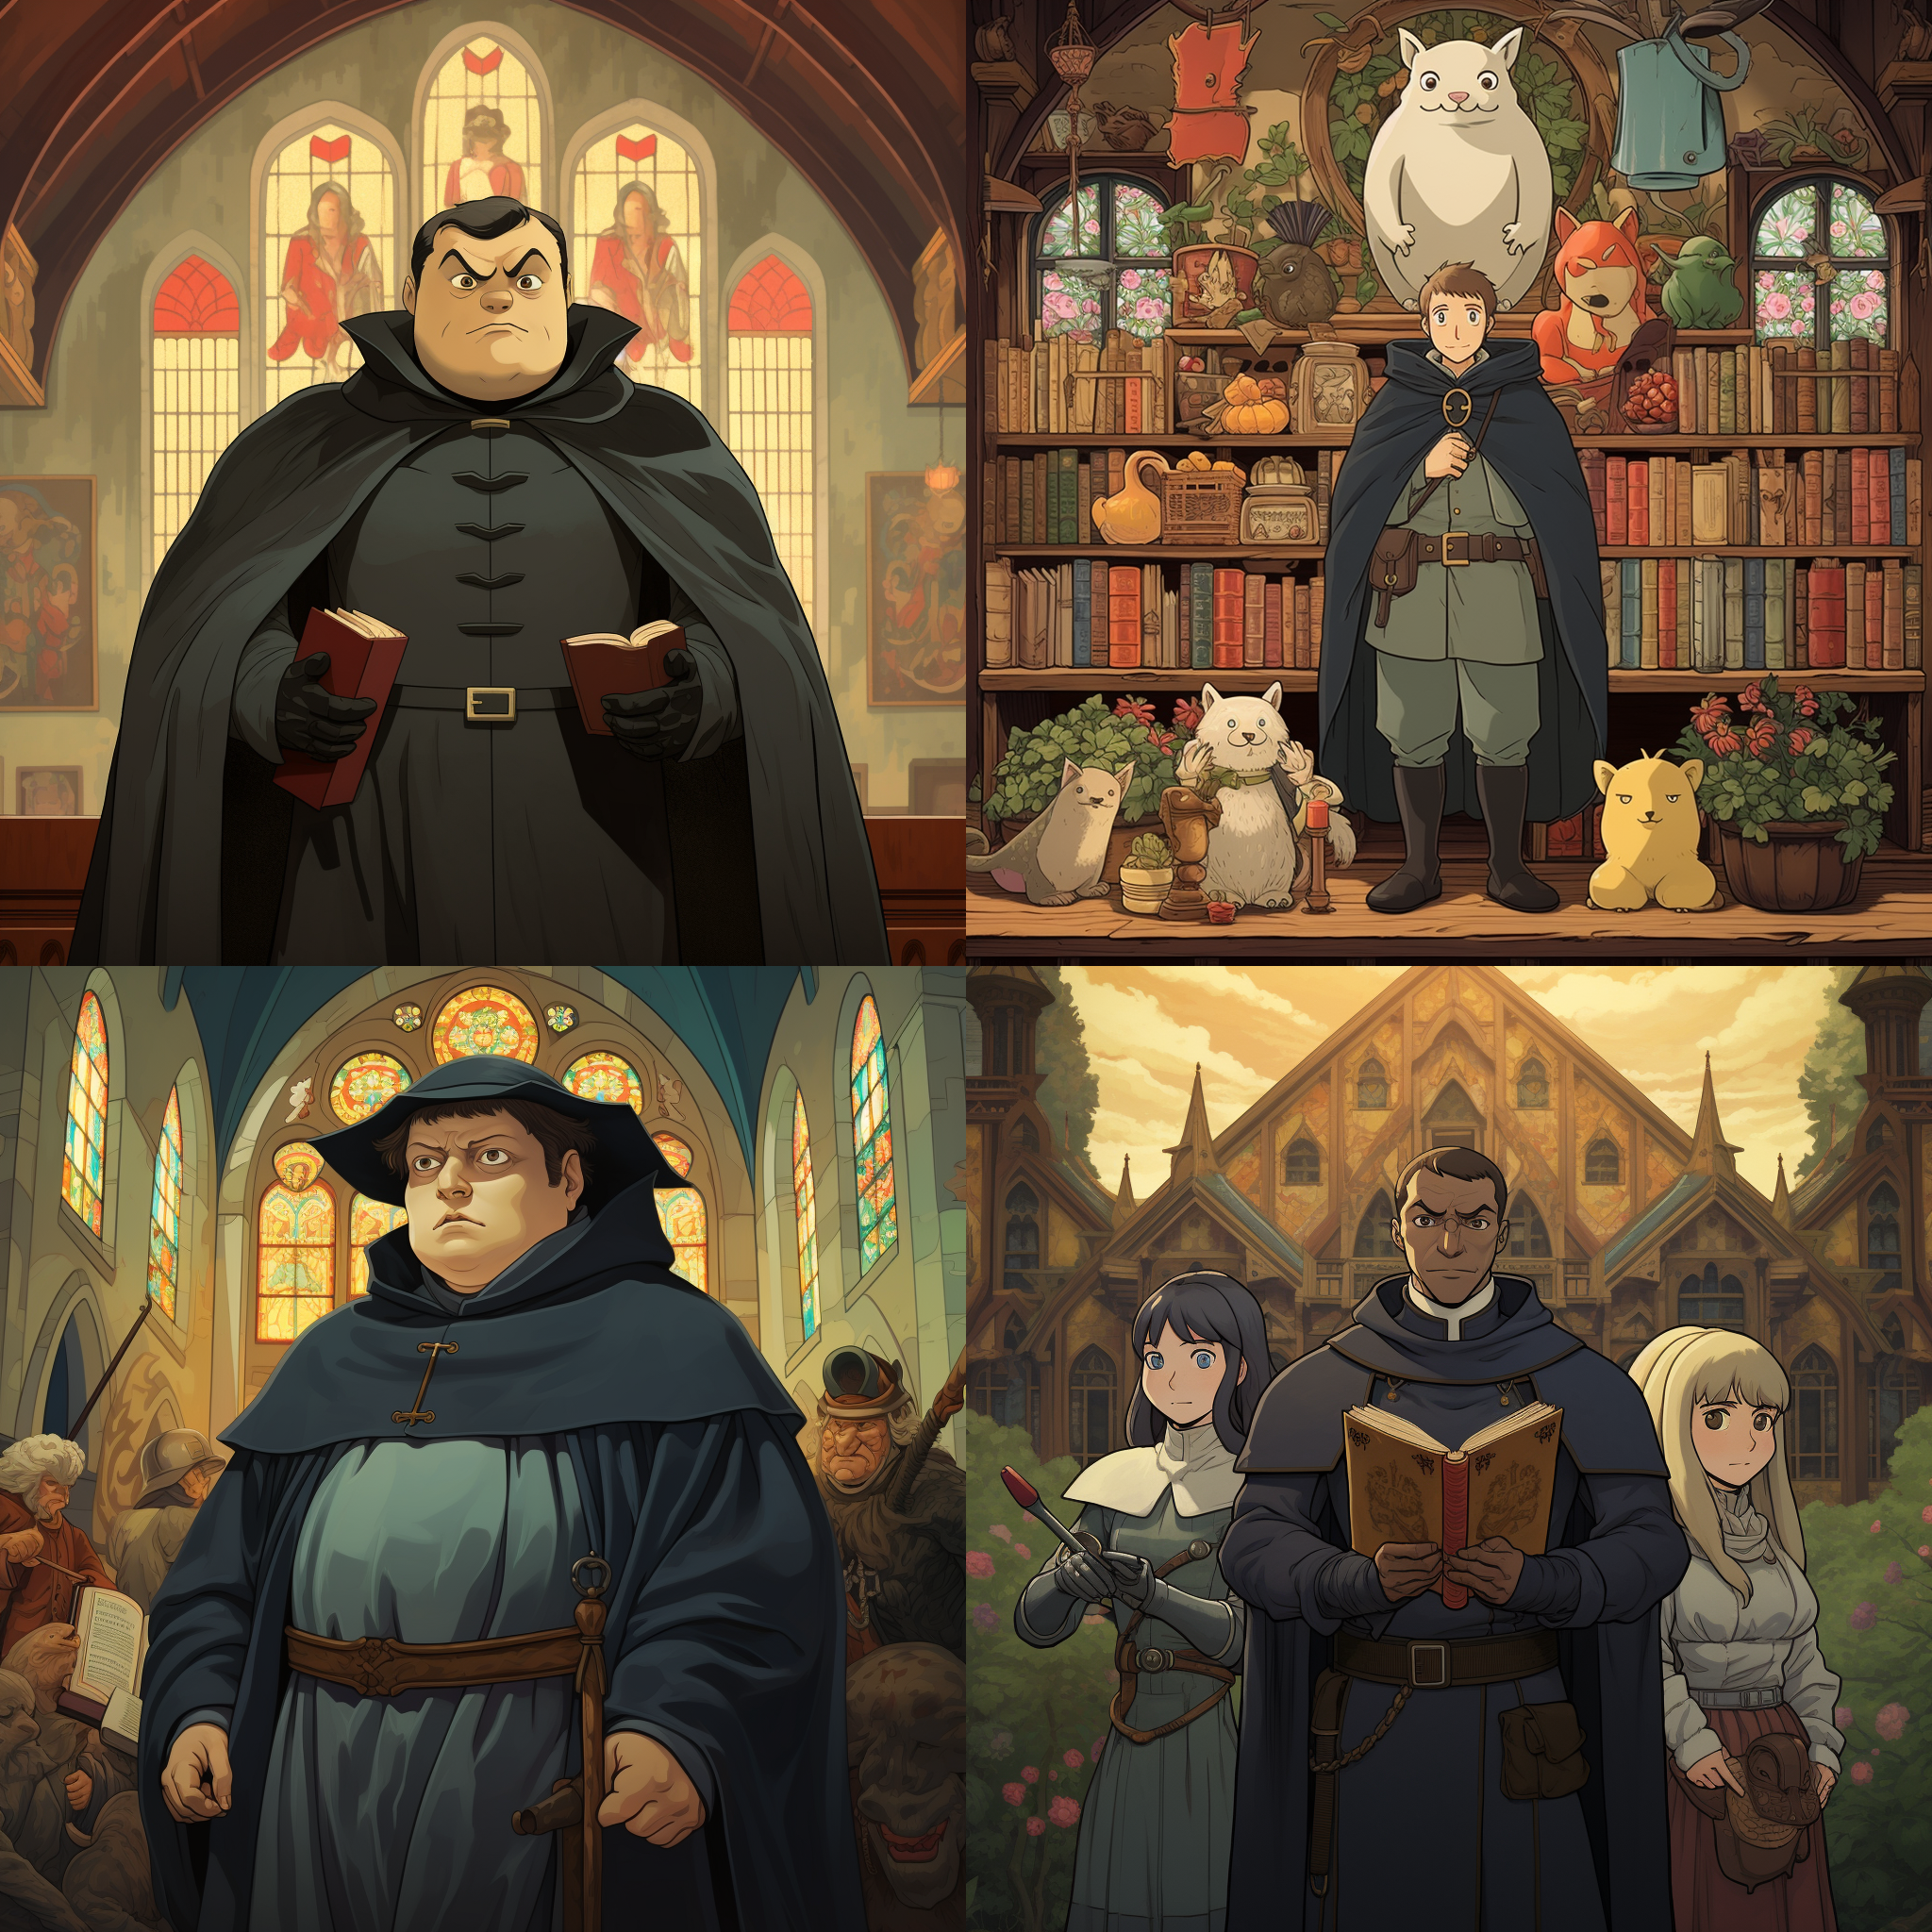
\includegraphics[width=4cm]{BilderFuerBA/Sonstiges/Martin_Luther_in_style_of_studio_ghibli}
	\end{minipage}
	\caption{Midjourney: Martin Luther in Stil von Ilya Kuvshinov, Banksy und Studio Ghibli}
	\label{MLinDreiStilen}
\end{figure}
\\
Zum Beispiel kann ich mit Midjourney ein Bild von Martin Luther Generieren Lassen in Stile von, Ilya Kuvshinov, Studio Ghibly oder Banksy generieren lassen wie zum Beispiel in Abbildung \ref{MLinDreiStilen}.
\\
Analog verhält es sich mit Texten die von ChatGPT erstellt werden können. Laut rolingstone.de klagen Schriftsteller wie George R. R. Martin gegen OpenAi, die Firma hinter ChatGPT.
\\
%https://www.gamestar.de/artikel/steam-geht-ki-vor-statement,3396779.html
Die dritte Meldung ist, das Steam, laut gamestar.de, Spiele mit KI-generierten Inhalten, aus ihrem Webshop löscht.
\\
Diese Drei Meldungen zeigen, das das Thema Urheberrecht noch nicht abgeschlossen ist, und ein Risiko in sich birg, ob es sinnvoll ist, KI-Systeme zu verwenden.

\chapter{Vorteile}
Während meiner Umsetzung des Videospielprototypens sind mir Folgende Vorteile aufgefallen
\section{Zeitersparnis}
Wenn die Einarbeitung in ein KI-Systeme geschehen ist, ist es möglich sehr viel Zeit zu sparen.
\\
Zum Beispiel habe ich 277 Dateien von Bilder in meinem Materialordner für den Dorfbaukasten. Darunter sind Holztexturen, Steintexturen, Texturen von Häuserfasaden und so weiter. Alle Texturen in meinem Verzeichnis, habe ich mindestens in dreifacher Ausführung, um Abwechslung in den Prototypen zu bekommen.
\\
Ich Persönlich besitze nicht die Fähigkeit zu zeichnen oder zu Malen.
\section{Gute und Günstige Ergebnisse}
%viele sachen kostenlos undsehr gute qualität, wie zum beispiel sound datein
Das testen von KI-System ist in der Regel kostenlos. Was dazu einlädt KI-Systeme auszuprobieren.  Aber auch. Menschen, die Menschen, Menschen, die mit diesem System sich erstmal beschäftigen möchten, bevor sie Geld investieren. Natürlich von erheblichem Vorteil ist.  

